\section{SQL pattern}


The \textit{proceedings} are the records of a conference.
ACM, as well as PVLDB, seeks to give these conference by-products a uniform,
high-quality appearance.  To do this, ACM / PVLDB has some rigid
requirements for the format of the proceedings documents: there
is a specified format (balanced  double columns), a specified
set of fonts (Arial or Helvetica and Times Roman) in
certain specified sizes (for instance, 9 point for body copy),
a specified live area (18 $\times$ 23.5 cm [7" $\times$ 9.25"]) centered on
the page, specified size of margins (2.54cm [1"] top and
bottom and 1.9cm [.75"] left and right; specified column width
(8.45cm [3.33"]) and gutter size (.083cm [.33"]).


\begin{figure}[h!] 
	\centering 
	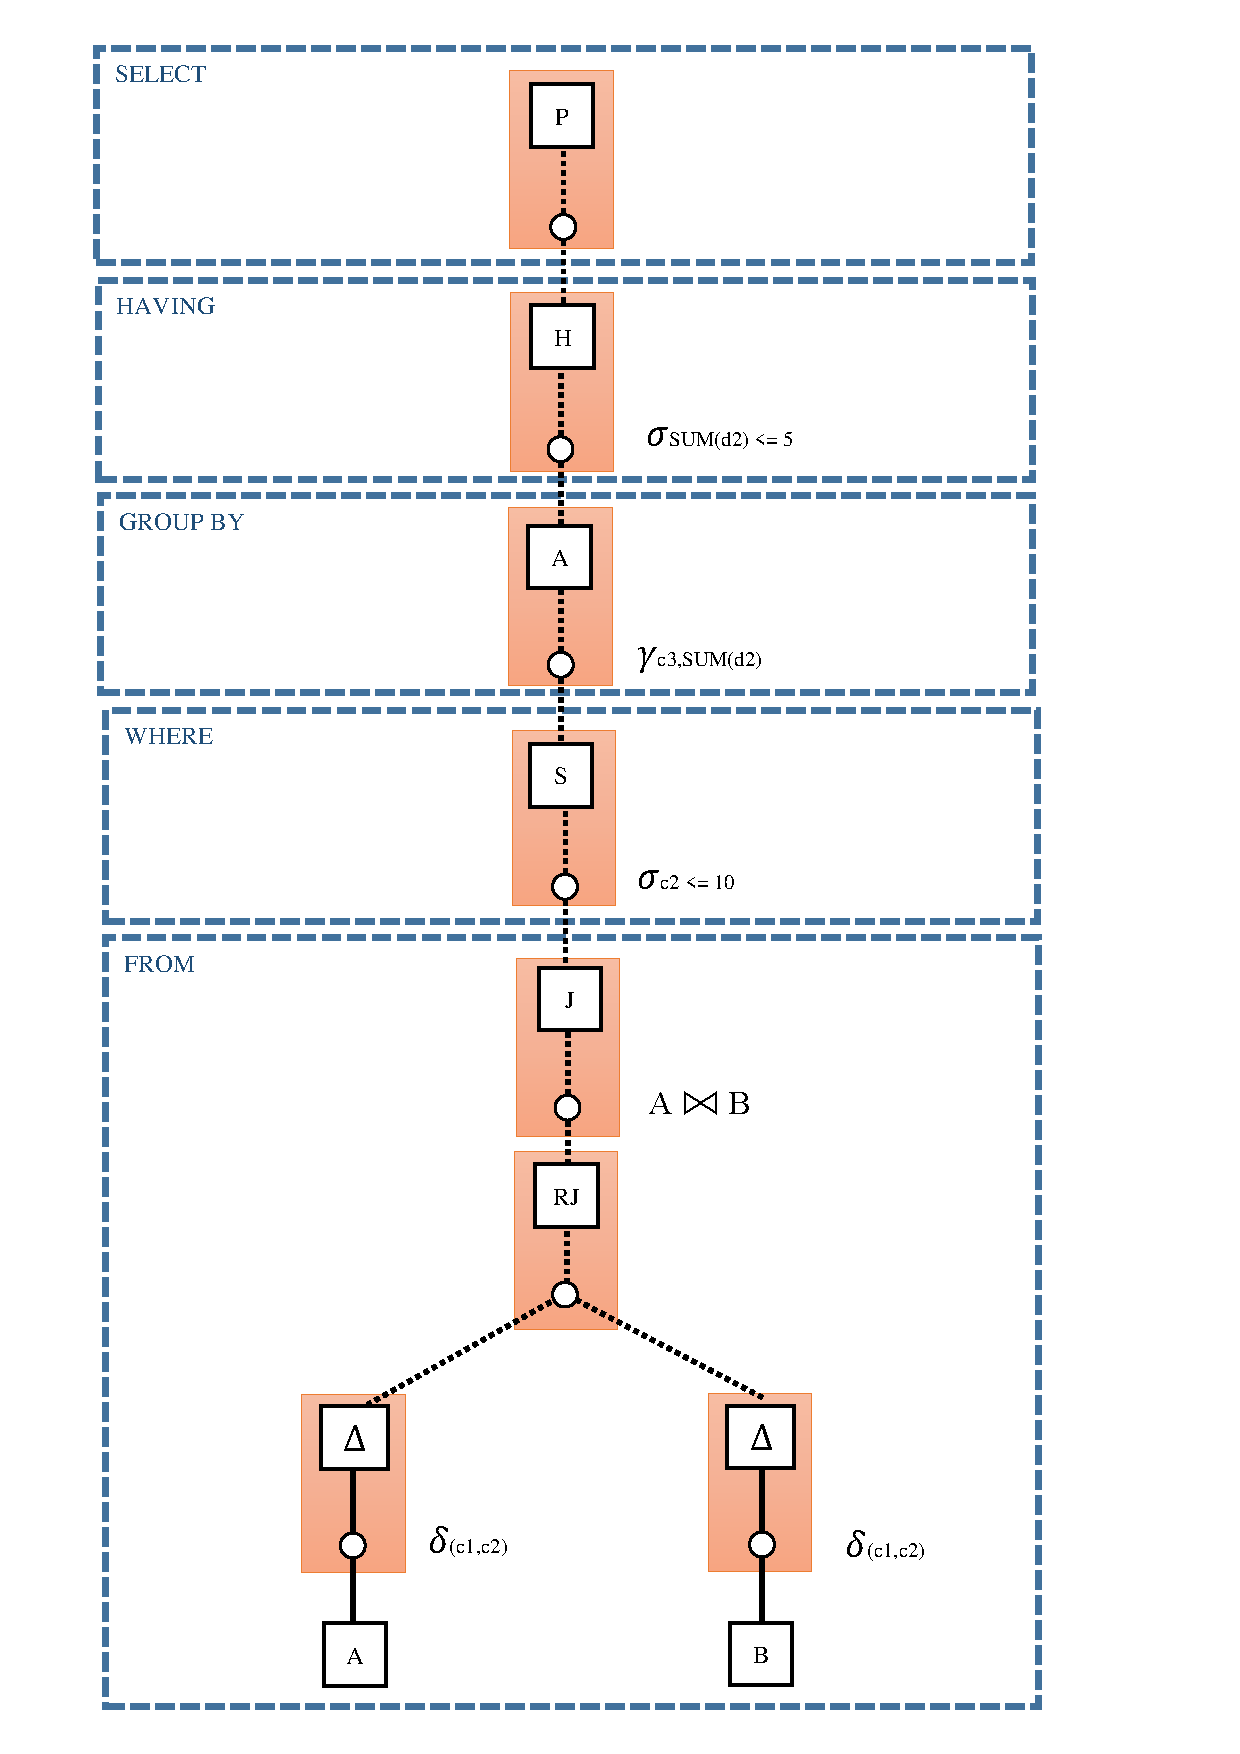
\includegraphics[width=\linewidth]{figures/SQLPattern}  
	\caption{SQL pattern} 
	\label{fig:sql_pattern} 
\end{figure} 

\subsection{Mapping}

	Clauses
	Evaluation order
	Mapping clauses -> view types



\subsection{Optimization}

Reorder
Merge 




The good news is, with only a handful of manual
settings\footnote{Two of these, the {\texttt{\char'134 numberofauthors}}
and {\texttt{\char'134 alignauthor}} commands, you have
already used; another, {\texttt{\char'134 balancecolumns}}, will
be used in your very last run of \LaTeX\ to ensure
balanced column heights on the last page.}, the \LaTeX\ document
class file handles all of this for you.

The remainder of this document is concerned with showing, in
the context of an ``actual'' document, the \LaTeX\ commands
specifically available for denoting the structure of a
proceedings paper, rather than with giving rigorous descriptions
or explanations of such commands.
